\documentclass[a4paper, 15pt]{report}
\usepackage[latin1]{inputenc}
\usepackage[italian]{babel}
%\usepackage[T1]{fontenc}
\usepackage{graphicx}
\usepackage{float}
\usepackage[centertags]{amsmath}
\usepackage{amsfonts}
\usepackage{amssymb}
\usepackage{amsthm}
\usepackage{newlfont}
\usepackage{fancyhdr}
\usepackage{tesisty}

% CUSTOM PACKAGE
\usepackage{hyperref}


%-------------------------------
% DEFINIZIONE DEGLI ENVIRONMENT
%-------------------------------

\newtheorem{obs}{Osservazione}[section]
\newenvironment{oss}
    {\begin{obs}\begin{normalfont}}
    {\hfill $\square \!\!\!\!\checkmark$ \end{normalfont}\end{obs}}

\newtheorem{pro}{Problema}[chapter]
\newenvironment{prob}
    {\begin{pro}\begin{normalfont}}
    {\hfill $\spadesuit$ \end{normalfont}\end{pro}}

\newtheorem{teor}{Teorema}[section]
\newenvironment{teorema}
    {\begin{teor}\textit }
    {\hfill  \end{teor}}

\newtheorem{defn}{Definizione}[section]
\newenvironment{de}
    {\begin{defn}\begin{normalfont}}
    {\hfill $\clubsuit$ \end{normalfont}\end{defn}}

% CUSTOM PACKAGE ENVIROMENT SET
\hypersetup{
	colorlinks=true,
	linkcolor=blue,
	filecolor=magenta,      
	urlcolor=cyan,
	pdftitle={Tesi Magistrale Alfano},
	pdfpagemode=FullScreen,
}

%-----------------------------
% CONFIGURAZIONE DELLA PAGINA
%-----------------------------

\hfuzz2pt % Don't bother to report over-full boxes if over-edge is < 2pt

\fancypagestyle{plain}{
\fancyhead{}\renewcommand{\headrulewidth}{0pt} } \pagestyle{fancy}
\renewcommand{\chaptermark}[1]{\markboth{\small CAP. \thechapter \textit{ #1}} {} }
\renewcommand{\sectionmark}[1]{\markright{\small  \thesection \textit{ #1}} {} }
\voffset=-20pt    % distanza tra il limite superiore del foglio e l'intestazione
\headsep=40pt     % distanza  l'intestazione ed il testo del corpo
\hoffset=0 pt     % misura equivalente al margine sinistro
\textheight=620pt % altezza del corpo del testo
\textwidth=435pt  % larghezza del corpo del testo
\footskip=40pt    % distanza tra il testo del corpo ed il pie' di pagina
\fancyhead{}      % cancella qualsiasi impostazione per l'intestazione
\fancyfoot{}      % cancella qualsiasi impostazione per il pie' di pagina
\headwidth=435pt  % larghezza del'intestazione e del pie' di pagina
\fancyhead[R]{\rightmark} \fancyfoot[L]{\leftmark}
\fancyfoot[R]{\thepage}
\renewcommand{\headrulewidth}{0.3pt}   % spessore della linea dell'intestazione
\renewcommand{\footrulewidth}{0.3pt}   % spessore della linea del pi�di pagina

\numberwithin{equation}{section}
\renewcommand{\theequation}{\thesection.\arabic{equation}}




%--------------------------
% MODIFICARE DA QUI IN POI
%--------------------------

\begin{document}

\dedicate{{
		Questa tesi � stata resa possibile dal contributo nella mia vita di tante persone, che giorno per giorno mi hanno sempre dato il loro sostegno, a voi dedico questa mia Tesi.\\
		Un ringraziamento speciale alla mia famiglia, in particolare a mia \textbf{Madre} e mio \textbf{Padre}: � grazie al vostro sostegno e incoraggiamento se oggi sono riuscito a raggiungere questo traguardo.\\
		La forza di arrivare qui, oggi, per� non � dovuta solo a loro, devo per forza ringraziare dell'affetto e il sostegno speciale da parte dei miei cari amici, che ogni giorno hanno condiviso con me gioie, sacrifici e successi, senza voltarmi mai le spalle, mi hanno dato la forza di arrivare a questo prezioso traguardo.
		\textbf{Filippo}, \textbf{Gabriele}, \textbf{Marta}, grazie di TUTTO.\\
		Un pensiero in particolare vola verso la mia dolce \textbf{\textit{Nicoleta}}, � sicuramente grazie all'affetto e le attenzioni che mi hai donato che sono riuscito a tenere dritto il timone ed arrivare qui oggi.
		Per terminare voglio ringraziare tutti i professori che negli ultimi 18 anni hanno guidato il mio cammino, loro che hanno sempre creduto in me e nelle mie capacit�. Un ringraziamento pi� speciale va per� alla mia professoressa e mentore \textbf{Beniamina Rauch} che fu la prima a vedere il mio potenziale e coltivarlo.\\
		Oltre a lei ringrazio il mio relatore \textbf{Daniele Carnevale} che in questi anni universitari, da quando mi ha conosciuto, ha sempre creduto in me e mi ha permesso di fare esperienze che mai avevo immaginato.\\ \\
		Un sentito grazie a tutti voi.\\
		Emanuele
		%TODO: Aggiungere firma con tavoletta frafica
}}

\corso{DELL'AUTOMAZIONE}
\titoloTesi{
	Sviluppo di algoritmi di controllo delle correnti nelle bobine poloidali di macchine per la fusione Tokamak, con riguardo al design	sistemico per la cooperazione tra sistemi embedded per l'attuazione, misurazione e centrali di controllo.
} \anno{2020/2021}
\relatore{Daniele Carnevale}
 \autore{Emanuele Alfano}
\correlatore{Marco Passeri}

\baselineskip=25pt

\intestazione

%------------------------------------------------
% INTRODUZIONE E RINGRAZIAMENTI (NON MODIFICARE)
%------------------------------------------------

\fancypagestyle{plain}{
\fancyhead{}\renewcommand{\headrulewidth}{0pt} } \pagestyle{fancy}
\renewcommand{\chaptermark}[1]{\markboth{\small Cap. \thechapter \textit{ #1}} {} }
\renewcommand{\sectionmark}[1]{\markright{\small  \S \thesection \textit{ #1}} {} }
\voffset=-20pt                         % distanza tra il limite superiore del foglio e l'intestazione
\headsep=40pt                          % distanza  l'intestazione ed il testo del corpo
\hoffset=0pt                           % misura equivalente al margine sinistro
\textheight=620pt                      % altezza del corpo del testo
\textwidth=435pt                       % larghezza del corpo del testo
\footskip=40pt                         % distanza tra il testo del corpo ed il pie' di pagina
\fancyhead{}                           % cancella qualsiasi impostazione per l'intestazione
\fancyfoot{}                           % cancella qualsiasi impostazione per il pie' di pagina
\headwidth=435pt                       % larghezza del'intestazione e del pie' di pagina
\fancyhead[R]{\rightmark} \fancyfoot[L]{\leftmark}
\fancyfoot[R]{\thepage}
\renewcommand{\headrulewidth}{0.3pt}   % spessore della linea dell'intestazione
\renewcommand{\footrulewidth}{0.3pt}   % spessore della linea del pi�di pagina

\pagenumbering{Roman}
\tableofcontents
\newpage

\pagenumbering{arabic}

\fancyhead[R]{Introduzione} \fancyfoot[L]{Introduzione}
\fancyfoot[R]{\thepage}

\chapter*{Ringraziamenti}
\addcontentsline{toc}{chapter}{Ringraziamenti}
\vspace{-8mm}
Questa tesi è stata resa possibile dal contributo nella mia vita di tante persone, che giorno per giorno mi hanno sempre dato il loro sostegno, a voi dedico questa mia Tesi.\\
Un ringraziamento speciale alla mia famiglia, in particolare a mia \textbf{Madre} e mio \textbf{Padre}: è grazie al vostro sostegno e incoraggiamento se oggi sono riuscito a raggiungere questo traguardo.\\
La forza di arrivare qui, oggi, però non è dovuta solo a loro, devo per forza ringraziare dell'affetto e il sostegno speciale da parte dei miei cari amici, che ogni giorno hanno condiviso con me gioie, sacrifici e successi, senza voltarmi mai le spalle, mi hanno dato la forza di arrivare a questo prezioso traguardo. \textbf{Filippo}, \textbf{Gabriele}, \textbf{Marta}, grazie di TUTTO.\\
Un pensiero in particolare vola verso la mia dolce \textbf{\textit{Nicoleta}}, è sicuramente grazie all'affetto e le attenzioni che mi hai donato che sono riuscito a tenere dritto il timone ed arrivare qui oggi.
Per terminare voglio ringraziare tutti i professori che negli ultimi 18 anni hanno guidato il mio cammino, loro che hanno sempre creduto in me e nelle mie capacità meritano tutta la mia gratitudine.\\
Un ringraziamento speciale va però alla mia professoressa e mentore \textbf{Beniamina Rauch} che fu la prima a vedere il mio potenziale e coltivarlo, so che ancora vegli su di me, non troverò mai le parole per ringraziarti abbastanza.\\
Oltre a lei ringrazio il mio relatore \textbf{Daniele Carnevale} che in questi anni universitari, da quando mi ha conosciuto ad oggi, ha sempre creduto in me e mi ha permesso di fare esperienze che mai avevo immaginato.\\ \\
Un sentito grazie a tutti voi e buona lettura.


\chapter*{Introduzione}
\addcontentsline{toc}{chapter}{Introduzione}
La tesi si colloca nell'ambito delle tecniche di controllo per impianti Tokamak, come FTU (Frascati Tokamak Upgrade), Proto-Sphera ed ITER (International Thermonuclear Experimental Reactor).\\
Essa è stata realizzata in collaborazione con il centro ricerche \textbf{ENEA} (Ente Nazionale per l’Energia e l’Ambiente) di Frascati e coordinato dal gruppo \textbf{CODAS} (COntrol and Data Acquisition System).\\
L'obiettivo finale del CODAS è di replicare in miniatura un intero impianto Tokamak, con particolare attenzione al prototipo dell'architettura software per il monitoraggio e controllo dell'esperimento.\\
In questa tesi viene discussa la creazione e lo sviluppo del prototipo della scheda embedded da usare per pilotare la corrente delle bobine magnetiche, generando così il confinamento magnetico del Plasma necessario alla reazione di fusione nucleare, presente all'interno del Tokamak.


\section*{Cos'è la Fusione Termonucleare?}
\addcontentsline{toc}{section}{Cos'è la Fusione Termonucleare?}
In fisica, per \textbf{Fusione Termonucleare}, si intende il processo mediante il quale i nuclei di due o più atomi vengono compressi tanto da far prevalere l’interazione forte sulla repulsione coulombiana, causando l'unione tra gli atomi e andando a formare così un nucleo la cui massa totale risulta minore della massa dei reagenti originali. La perdita di massa ha come conseguenza la liberazione di un’elevata quantità di energia, la quale conferisce al processo caratteristiche fortemente esotermiche.\\
La massa mancante viene trasformata in energia in accordo con l’equazione di Einstein:
\begin{center}
	$E = (m_r - m)c^2$
\end{center}
Dove $ m_r $ è la massa dei reagenti e $ m $ è la massa risultante.\\
Il processo di \textbf{Fusione Nucleare} avviene naturalmente all'interno delle stelle e trasforma l'\textit{idrogeno} (di cui sono composte) in \textit{elio}.\\
L'energia nucleare prodotta a seguito di questa reazione è elevatissima e per tale motivo risulta di forte interesse per la civiltà umana sviluppare tecniche sofisticate che ne permettano la raccolta in maniera controllata.\\
Tra i vantaggi di questa tecnologia troviamo sia motivi economici che ambientali e i principali possono essere sintetizzati in:
\begin{description}
	\item [Combustibile semi-inesauribile]:\\
	      Il combustibile (idrogeno e/o deuterio) è praticamente inesauribile ed è a disposizione di tutte le nazioni che abbiano uno sbocco sul mare. Il deuterio può essere estratto dall'acqua, anche se con costi energetici non indifferenti;\\
	      per fare un esempio, un ditale pieno di deuterio equivale a 20 tonnellate di carbone in termini di energia.\\
	      Un lago di medie dimensioni contiene deuterio sufficiente a rifornire una nazione di energia per secoli utilizzando la fusione nucleare (ovviamente supponendo di sfruttarlo tutto).
	\item [Rischi di Contaminazione grave sono \underline{nulli}]:\\
	      Nessuna possibilità di incidenti come quelli di Černobyl' o di Three Mile Island in quanto il reattore non contiene sostanze radioattive come l'uranio o le scorie di fissione.\\
	      In oltre, possibili incidenti, come fughe di trizio o perdite di liquido refrigerante, avrebbero un impatto ambientale e radiativo molto più contenuto e temporaneo.
	\item [Assenza di inquinanti ambientali]:\\
	      Il processo di fusione, durante il quale gli atomi di idrogeno vengono fusi per creare elio, non rilascia nessun elemento inquinante da combustione (ad esempio anidride carbonica) e per tanto nessun residuo può essere immesso nell'atmosfera impedendo il riscaldamento del pianeta tramite l'effetto serra.
	\item [Nessuno prodotto derivato è adatto a fini Bellici]:\\
	      La mancanza di materiale radioattivo residuo, impedisce l'utilizzo dei reattori per la produzione di materiale per scopi bellici o terroristici, come proiettili radioattivi o materiale fissile per bombe nucleari.
	\item [Livelli lievi di radiottività residua]:\\
	      Il processo di fusione può rendere radioattivi solo i materiali che compongono il Tokamak e i gas usati per il Plasma, ma entrambi gli elementi possiedono un tempo di decadimento alquanto breve, il ché implica che i rifiuti radioattivi hanno una scarsa durata nel tempo, in oltre le radiazioni prodotte non sono a energie elevatissime, semplificandone il contenimento attraverso contenitori schermati più economici e sicuri.
\end{description}
\noindent
Questi e molti altri motivi rendono lo sviluppo di metodi per catturare l'energia da \textbf{Fusione Nucleare} con attraverso processi controllati di grande interesse per tutta la civiltà umana, essa potrebbe infatti essere la chiave per preservare l'ambiente del nostro pianeta e fornire al temo stesso l'energia di cui l'umanità necessita.\\
In questa tesi faremo riferimento ad una classe di impianti sperimentali per la \textbf{Fusione Nucleare Controllata}, detti "\textbf{Impianti Tokamak}". \'E doveroso specificare che essi sono solo uno dei tanti design su cui attualmente si fa ricerca e sviluppo nel mondo, ma tra le varie proposte essi sembrano essere i più promettenti per aprire le porte a questa rivoluzione, poiché il principio di base è la replica delle condizioni che generano la fusione all'interno in una stella.\\
Tolte le difficoltà tecniche per le quali infatti è ancora una tecnologia in sviluppo, abbiamo la sicurezza sperimentale della fattibilità del processo, la nostra stessa civiltà non esisterebbe se il Sole non producesse questa forma di energia al suo interno.
\newpage

\section*{Struttura di un Tokamak}
\addcontentsline{toc}{section}{Struttura di un Tokamak}
Un \textbf{Tokamak}\footnote{Tokamak è l'acronimo russo per "camera toroidale magnetica"} è una macchina di forma toroidale (a ciambella) in cui un gas (solitamente idrogeno) viene portato nello stato di Plasma e mantenuto coeso e lontano dalle pareti interne grazie ad un campo magnetico creato da elettromagneti esterni alla camera.
\begin{figure}[H]
	\centering
	\caption[Sezione di un Tokamak]{Sezione di un Tokamak}
	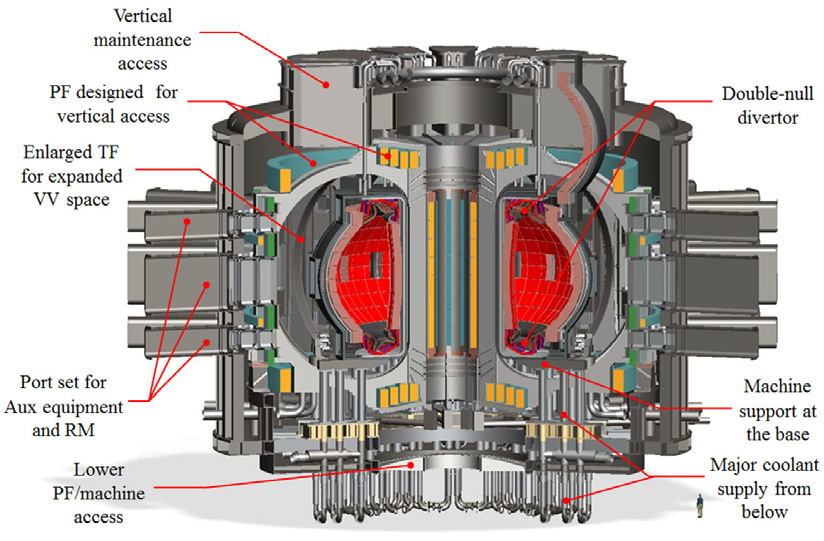
\includegraphics[width=0.65\textwidth]{Introduzione/K-DEMO_device_core_design_features.jpg}
\end{figure}

\noindent
La forma del Tokamak a \textit{toro} è studiata per permettere alle particelle del Plasma di muoversi all'interno del campo magnetico, creato all'esterno delle pareti (\textit{Esterno del Vessel}) in un moto circolare.\\
Questo movimento avviene poiché le particelle del Plasma sono per definizione cariche, e in quanto tali, se immerse in un campo magnetico esse tendono a muoversi seguendo una traiettoria elicoidale (detta anche \textit{moto di ciclotrone}) attorno alle linee del campo magnetico, che in questo caso sono chiuse e contenute all'interno della sezione del Tokamak (\textit{Interno del Vessel}).\\
L'uso di una confinazione magnetica di questo Plasma è dovuta all'impossibilità, per qualunque materiale, di resistere alle enormi temperature raggiunte dal Plasma durante la fusione in caso di un contatto diretto.\\

\noindent
La forma scelta per i Tokamak a Toro ha motivazioni fisiche, che discendono principalmente dall'equazione di Larmor. L'equazione descrive la distanza massima oltre il quale una particella carica non può allontanarsi da una linea di campo magnetico, definendo un limite superiore per lo spazio di contenimento delle particelle; questa distanza è detto appunto \textit{raggio di Larmor}:\\
\begin{vwcol}[widths={0.3,0.7}, sep=8mm, rule=1px]
	\begin{empheq}[box=\mathCalc]{equation*} \label{eq:Larmor}
		{\displaystyle \,\rho ={\frac {mv_{\perp }}{Ze\,B}}}
	\end{empheq}
	\newpage % con wcol, le colonne sono "pagine"
	\begin{spacing}{1.25}
		{\footnotesize
			$ {\displaystyle v_{\perp }} $ è la velocità della particella perpendicolare al campo magnetico.\\
			$ {\displaystyle m} $ è la sua massa.\\
			$ {\displaystyle B} $ è l'intensità del campo magnetico.\\
			$ {\displaystyle Ze} $ è la carica del portatore.
		}
	\end{spacing}
\end{vwcol}
\noindent
L'equazione vale anche in presenza di un campo magnetico curvo, se questa curva è chiusa si ottiene che la particella è confinata in uno spazio di volume finito ma rimane comunque libera ruotare all'infinito, accumulando così energia.\\
\'E stata scelta la geometria del \textbf{Toro} per rendere questa linea di campo una circonferenza esatta, la quale semplifica enormemente delle complesse equazioni fluido-dinamiche applicate al Plasma.\vspace{-5mm}
\begin{figure}[H]
	\centering
	\caption[Geometria di un Toro]{Geometria di un Toro}
	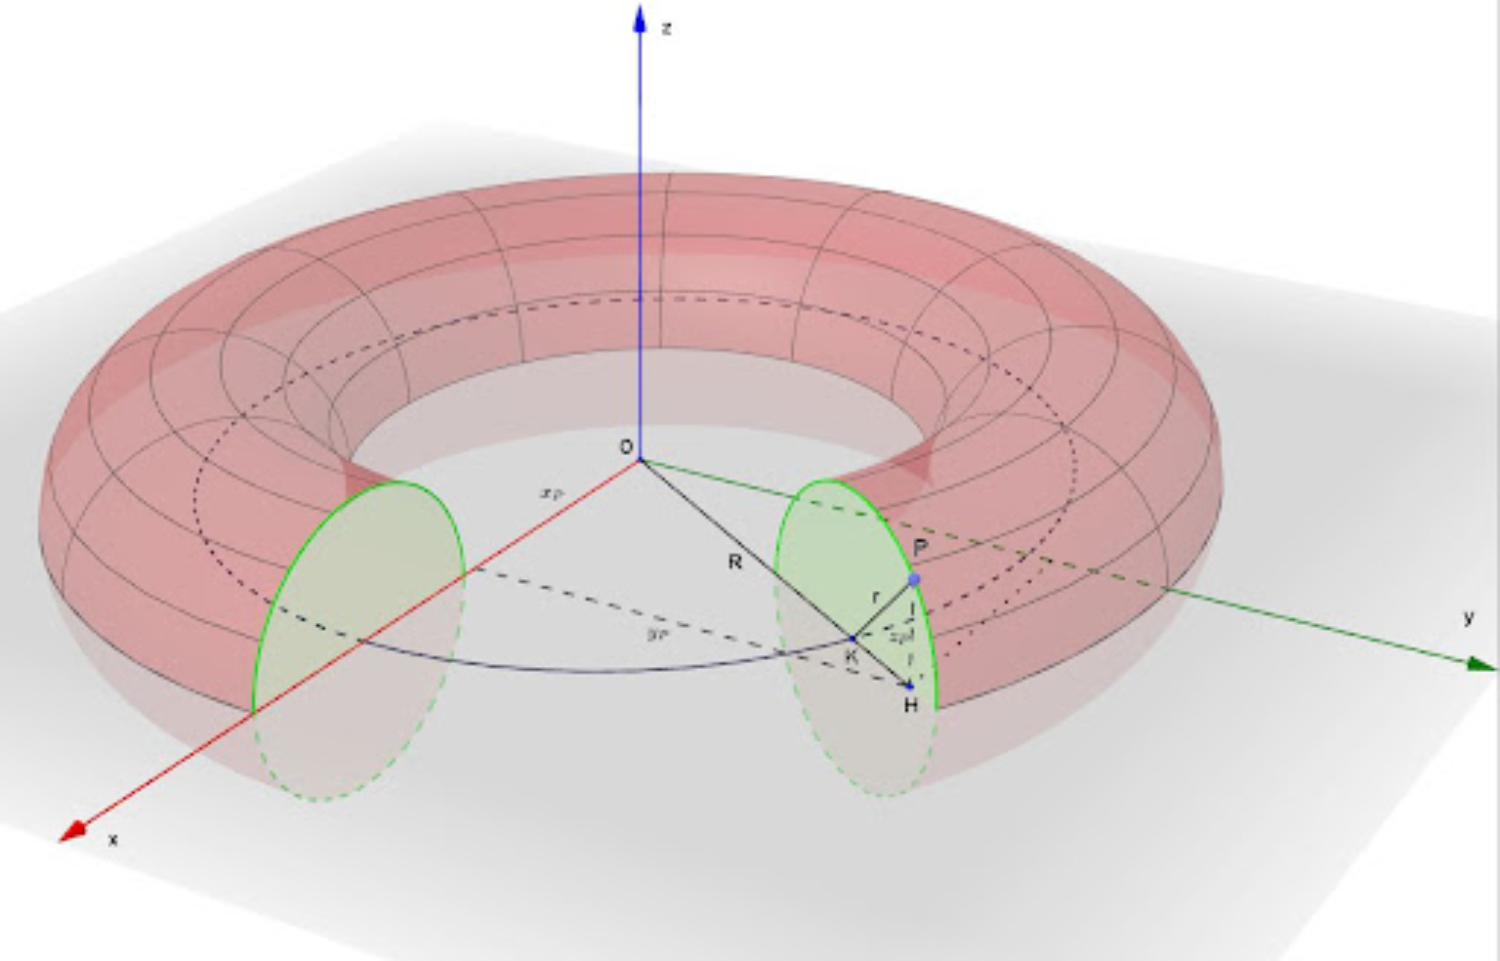
\includegraphics[width=0.65\textwidth]{Introduzione/toro-big.png}
\end{figure}\vspace{-8mm}
\noindent
In sintesi un Tokamak è un impianto progettato per creare questo confinamento magnetico in maniera efficace e sicura, e ha la forma più consona per realizzare questo processo.\\
Oltre al mero contenimento però, il secondo obiettivo è quello di compattare il Plasma su se stesso (aumentando la forza del campo magnetico $ B $), così da avvicinare di più gli atomi tra loro (l'aumento di $ B $ causa una riduzione di $ \rho $).\\
Questo aumento di pressione, unito alle alte energie immesse nel Tokamak (la cui temperatura è \textbf{di decine di volte} superiore a quella della superficie del sole) aumentano le probabilità di scontro tra gli atomi, e quindi inizio di un processo di fusione tra essi. 

\section*{Obiettivi della Tesi}
\addcontentsline{toc}{section}{Obiettivi della Tesi}
Il progetto complessivo portato avanti dall'ENEA prevede la realizzazione di prototipi a più livelli di un sistema Tokamak.\vspace{-4mm}
\begin{figure}[H]
	\centering
	\caption[Architettura Complessiva Progetto ENEA]{Architettura Complessiva Progetto ENEA}
	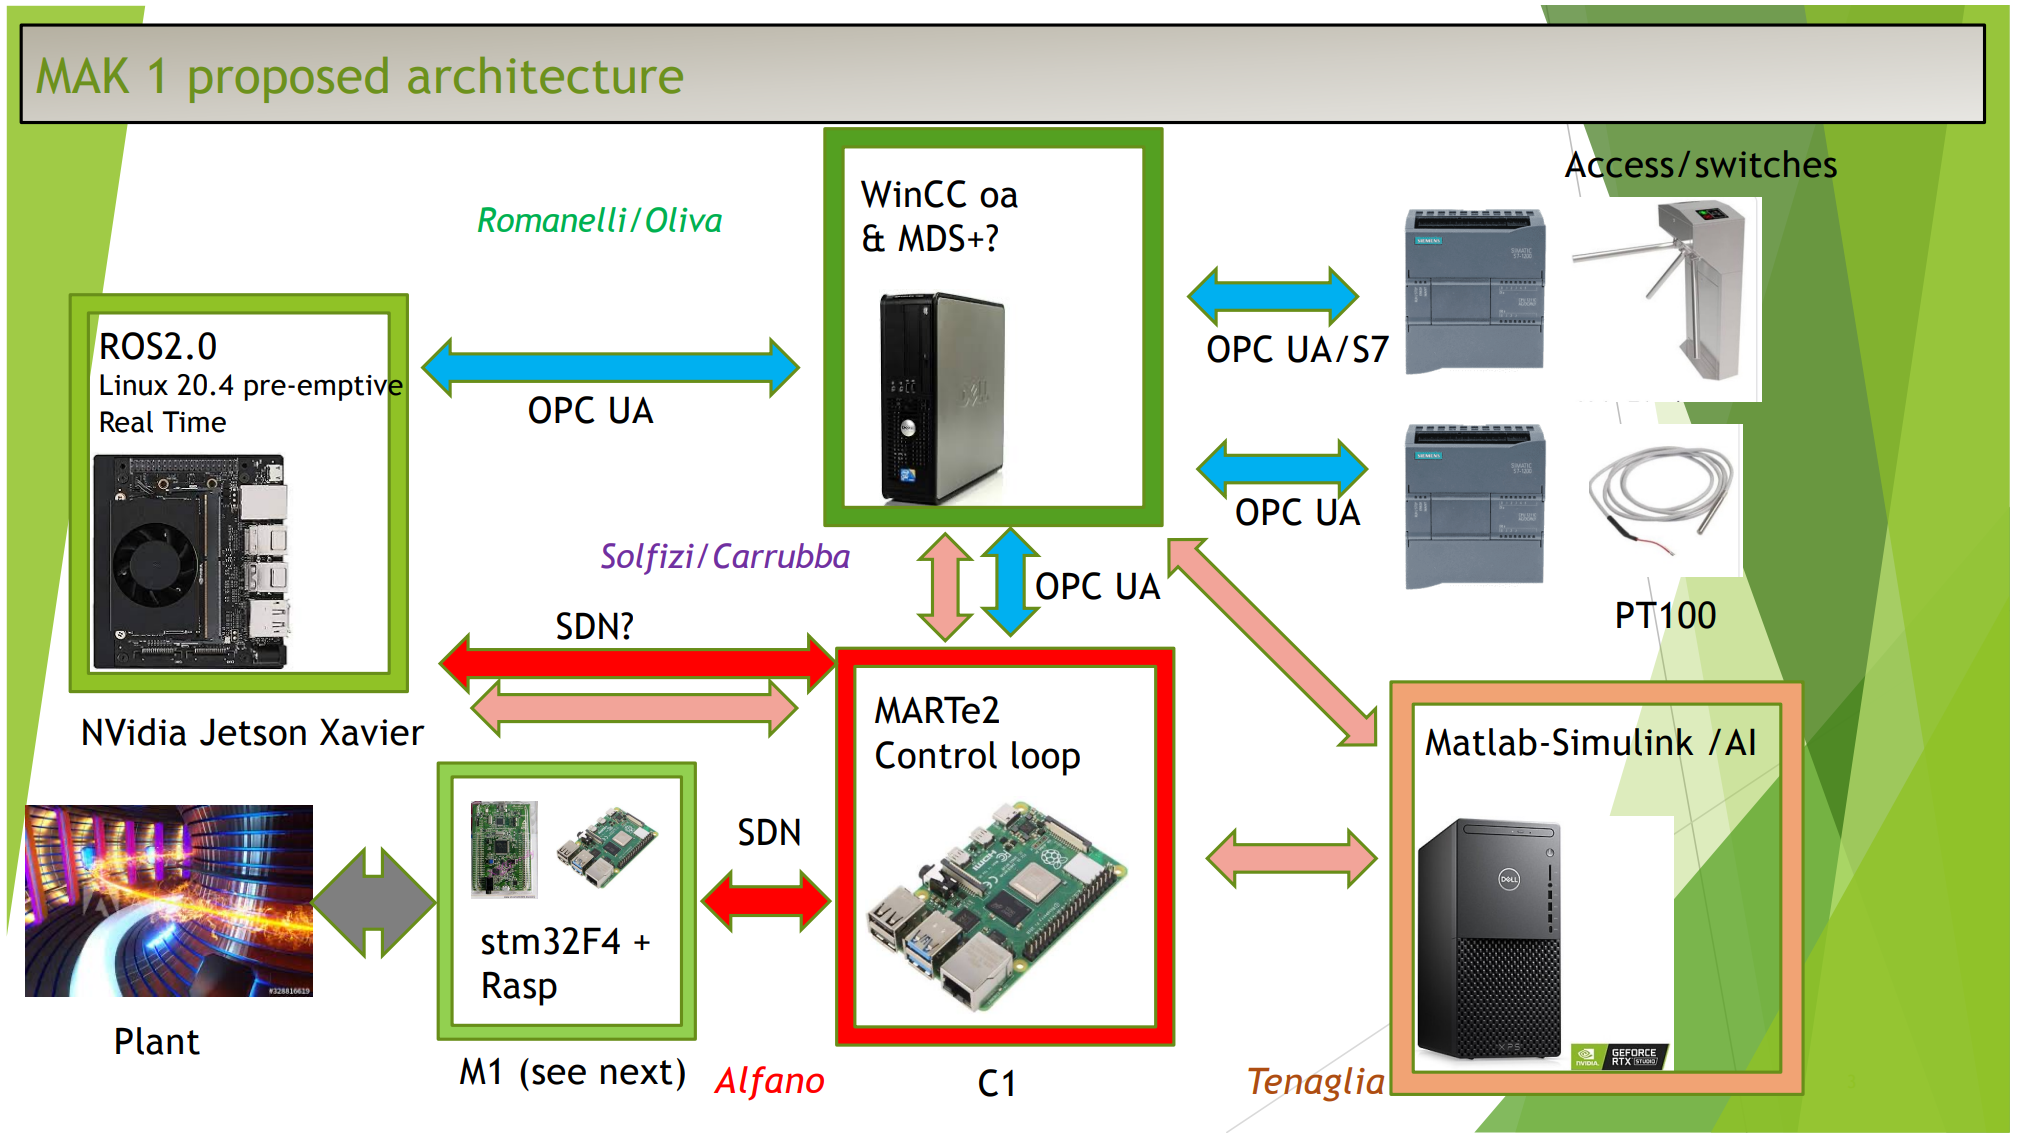
\includegraphics[width=\textwidth]{Introduzione/ArchitetturaComplessiva.png}
\end{figure}\vspace{-8mm}
\noindent
La mia parte di progetto ({\color{red}Alfano}) consiste nello sviluppare e realizzare una una scheda embedded.\\
Essa dovrà pilotare la corrente nelle bobine dell'impianto Tokamak ed essere in grado di ricevere e inseguire i riferimenti per la corrente di Plasma attraverso la rete di interconnessione tra i dispositivi, basata sul Framework di \MARTe. (argomento trattato con dettaglio nella tesi)\\
Il controllo realizzato punta a inseguire il riferimento richiesto con un errore nullo.\\
In fine il dispositivo deve essere in grado di comunicare in real-time l'attuale stato del sistema al resto della rete, per permettere una diagnostica in tempo reale dell'andamento dell'impianto.\\

\fancyhf{} %elimina header/footer vecchi


\fancyhead[R]{\rightmark} \fancyhead[L]{\leftmark}
\fancyfoot[R]{\thepage}





%---------------------
% INCLUSIONE CAPITOLI
%---------------------

\chapter{Alcune regole fondamentali}
\label{chap:fond}

\begin{minipage}{12cm}\textit{Se lo si desidera, utilizzare questo spazio per inserire un breve riassunto di ci\`o che verr\`a detto in questo capitolo. Inserire solo i punti salienti.}
\end{minipage}

\vspace*{1cm}

\section{Come iniziare}
\label{sec:iniziare}

La tesi va scritta partendo dall'indice. Dopo aver avviato il lavoro,
lo studente deve fare uno sforzo di qualche giorno per scrivere  un
indice quanto pi\`u accurato e strutturato possibile della
relazione. L'indice va poi discusso col relatore, possibilmente prima
di incominciare a scrivere, in quanto esso influisce fortemente sul
tono da tenere nella scrittura.

L'indice pu\`o essere preparato con l'ausilio di LaTeX semplicmente
impostando le varie sezioni e affidandosi al comando
\verb1\tableofcontents1 che genera automaticamente l'indice in cima
alla tesi. Successivamente, durante la scrittura, i vari capitoli
vuoti verranno rimepiti.

ATTENZIONE a non cadere nell'errore di sottostimare il proprio lavoro
e iniziare a scrivere cose scopiazzate qua e l\`a. La relazione deve
corrispondere ad una descrizione dettagliata del lavoro fatto (\`e
questa la cosa pi\`u importante da documentare, in aiuto del relatore
e in aiuto dei tesisti che eventualmente proseguiranno il
lavoro). Tutto ci\`o che non riguarda il lavoro fatto sar\`a una parte
introduttiva scritta alla fine, anche di corsa, e di scarso
interesse. A volte gli studenti fanno l'errore di cominciare a
scrivere un lungo trattato su cose che non sono farina del loro
sacco. Quando arrivano alla vera e proria descrizione del loro lavoro,
ormai la tesi \`e gi\`a troppo lunga e sacrificano proprio quella
parte, la pi\`u importante, per mancanza di tempo e di
energie. Quindi: cominciate {\rm sempre} a scrivere dalla parte
centrale dell'indice della tesi, e poi man mano aggiungete le parti
introduttive. La tesi non viene scritta di getto dall'inizio alla
fine, come in una operazione di copiatura, ma nasce dalla sua parte
centrale, quella pi\`u importante, e poi man mano si gonfia come un
palloncino, eventualmente vedendo, durante la propria crescita, delle
revisioni dell'indice e dei cambi strutturali (quali lo swap di due
capitoli o lo spostamento di un intero capitolo in appendice)
nell'interesse della chiarezza e dell'organicit\`a del documento.


\section{Questioni di impostazione}
\label{sec:impostazione}

In questa sezione vengono commentate alcune questioni estetiche e di
forma legate alla tesi.

\subsection{La terza persona}

La tesi va scritta usando la terza persona, per quanto possibile, tranne casi veramente eccezionale. In inglese \`e piuttosto standard usare la prima persona (plurale) in testi tecnici. In italiano no.

\subsection{La lingua}

L'impostazione della lingua (italiana) \`e fondamentale perch\'e le parole vengano spezzate correttamente dal LaTeX quando deve andare a capo. Tale impostazione funziona soltanto se il LaTeX che si utilizza \`e corredato dei corrispondenti files di stile.

\subsection{La punteggiatura}
\label{sec:puntegg}

La punteggiatura va {\bf sempre} attaccata alla parola precedente e
staccata (con uno spazio) dalla parola seguente (a parte le virgolette
aperte per le quali vale la regola opposta).

\subsection{Gli accenti}
\label{sec:accenti}

In LaTeX non \`e possibile scrivere un carattere accentato semplicemente riportandolo nel codice TeX. Per farlo si deve usare un comando particolare: \verb1\`1. Ad esempio \verb1\`e1 produrr\`a \`e.\\

NOTA!!! Il carattere `` ` '' \`e diverso dal carattere `` ' ''! Col primo si ottiene \`e, col secondo \'e!\\
In Linux questo ``accento obliquo'' \`e ottenibile utilizzando la combinazione di tasti ALTGR+'. In ambiente Windows si consiglia di utilizzare la Mappa Caratteri.\\

{\bf ATTENZIONE AGLI ACCENTI}: Da un punto di vista grammaticale,
tutte le parole accentate italiano 
hanno accento grave, ovvero dall'alto verso il basso, eccezion fatta
per la lettera `` e '' che pu\`o avere sia accento acuto che grave a
seconda della parola. Pi\`u specificatamente, le `` e '' accentate sono
quasi tutte acute, a parte due parole: `` \`e '' e `` cio\`e '' (infatti
perch\'e, poich\'e, affinch\'e, etc. hanno tutte l'accento
acuto). Un'ultima osservazione va fatta per la lettera `` i ''
accentata: la si ottiene con la sequenza \verb1\`{\i}1 che d\`a il
seguente risutato: \`{\i}.

\subsection{Le virgolette}

Le virgolette aperte si ottengono con la sequenza \verb1``1 mentre
quelle chiuse si ottengono con la sequenza \verb1''1 oppure con il
carattere \verb1"1.

\subsection{Posizione delle figure}

Il LaTeX posiziona le figure automaticamente, questo significa che
esse non appariranno sempre dove ci aspettiamo di vederle. \`E dunque
fondamentale riferirsi alle figure con il comando
\verb1In figura~\ref{fig:mylabel}1 che fa riferimento ad una label
specificata dentro la figura tramite il comando
\verb1\label{fig:mylabel}1 e che consente di riferirsi alla figura con
il suo numero e senza riferimenti legati al layout del testo (tipo:
``qui sotto'' oppure `` in cima alla pagina'', oppure ``nella pagina
seguente'', etc.)

\subsection{Caption e note a pi\'e di pagina}

Le note a pi\'e di pagina 
si ottengono semplicemente digitando 
\verb1\footnote{Questo \`e il testo.}1 attaccato alla lettera
precedente (questo \`e ci\`o che 
risulta\footnote{Questo \`e il  testo.}).

Sia per le note che per le (o legende) delle figure, \`e necessario
sempre partire con la lettera maiuscola e terminare con un punto.



\chapter{Basi di latex}
\label{chap:basi}

\begin{minipage}{12cm}\textit{Se lo si desidera, utilizzare questo spazio per inserire un breve riassunto di ci\`o che verr\`a detto in questo capitolo. Inserire solo i punti salienti.}

\end{minipage}

\vspace*{1cm}

\section{Sezionamento}
\label{sec:sezioni}

Per suddividere la tesi in LaTeX in vari sottocapitoli \`e sufficiente
usare dei comandi specifici. In particolare \verb1\chapter{titolo}1
inizia un nuovo capitolo, \verb1\section{titolo}1 un nuovo
sottocapitolo e \verb1\subsection{titolo}1 un nuovo
paragrafo. Tendenzialmente non occorre scendere ulteriormente nella
struttura, in ogni caso esiste eventualmente anche il comando
\verb1\subsubsection{titolo}1.\\ 

Il modello della tesi \`e organizzato in modo da mantenere un unico
file principale con tutti i comandi di base (impaginazione, nuovi
environment...) denominato Tesi.tex, in modo che una volta modificato
questo non sia pi\`u necessario mettervi mano, e un file distinto per
ogni capitolo, denominato capitoloN.tex. Si consiglia di mantenere
tale sistema in quanto semplice e allo stesso tempo efficiente, specie
in fase di correzione.\\ 

Nota bene: non occorre compilare ogni singolo capitoloN.tex, basta
compilare Tesi.tex, che include tutti i capitoli scritti! L'importante
\`e che ogni nuovo capitolo creato venga segnalato nel file Tesi.tex
nella parte di ``inclusione capitoli'' con la direttiva
\verb1include{capitoloN}1 (si noti che non \`e necessario inserire
l'estensione .tex).\\ 



\section{Le immagini}
Per inserire immagini in latex si utilizza l'ambiente \texttt{figure}:\\

\begin{verbatim}
\begin{figure}[POS]
        \centering
        \includegraphics[width=Xcm]{imgs/NOME.eps}
        \caption{Descrizione della figura.}
        \label{fig-label-figura}
\end{figure}
\end{verbatim}

\vspace*{1cm}

\noindent dove al posto di POS va inserita una lettera a scelta tra \textit{h}, \textit{t} e \textit{b} che indicano in che posizione ``suggerire'' a LaTeX di inserire l'immagine, rispettivamente 'here', 'top' e 'bottom'. L'utilizzo pi\`u tipico \`e quello con la lettera \textit{h}, che indica di inserire l'immagine, se possibile, nella posizione corrente. Al posto di X va inserita la dimensione desiderata per l'immagine (in questo caso, width, per quanto riguarda la dimensione orizzontale; per specificare l'altezza bisogna utilizzare height). Caption indica il testo che verr\`a inserito sotto la figura e label come ci si riferir\`a alla figura. In questo caso, avendo definito la label di quest'immagine ``fig-label-figura'', per riferirsi ad essa (es.: ``vedi figura 2.4''...) nel file tex si sarebbe utilizzato il comando \verb1\ref{fig-label-figura}1.

Si consiglia di usare immagini in formato EPS in quanto standard. Matlab permette di esportare grafici in tale formato, cos\`i come la maggior parte dei programmi di editing grafico per Linux o in generale open-source (GIMP, Dia...). Nel mondo Windows, Adobe Photoshop permette di esportare come EPS.\\

Nel caso si voglia disporre la figura ruotata di 90 gradi a pagina intera (per esempio per riportare grossi grafici di Matlab), si usi l'ambiente \texttt{sidewaysfigure}:\\


\begin{verbatim}
\begin{sidewaysfigure}[POS]
        \centering
                \includegraphics[width=Xcm]{imgs/NOME.eps}
        \caption{Descrizione della figura.}
        \label{fig-label-figura}
\end{sidewaysfigure}
\end{verbatim}

\vspace*{1cm}

\section{Le tabelle}
La sintassi con cui si inseriscono le tabelle \`e la seguente:\\
\begin{verbatim}
\begin{center}
\begin{tabular}{COLS}
CONTENT
\end{tabular}
\end{center}
\end{verbatim}

\noindent dove al posto di COLS va inserita la struttura delle colonne. Si tratta di una stringa composta dai caratteri l, r e c, che stanno rispettivamente per left, right e centre. Il carattere | impone di tracciare una divisione verticale. Per esempio scrivere ``lr|c'' equivale a chiedere a LaTeX di disegnare una tabella la cui prima colonna sia allineata a sinistra, la seconda a destra e la terza centrata, con una riga di separazione verticale tra la seconda e la terza colonna.\\
Al posto di CONTENT vanno inseriti i dati da mettere nella tabella: per spostarsi tra le colonne si usa il carattere \verb1&1, per iniziare una nuova riga si usa \verb1\\1. Per esempio, usando la struttura delle colonne definita precedentemente, scrivere ``\verb1a & b & c\\1'' equivale a mettere a nella prima colonna, b nella seconda e c nella terza, iniziando quindi una nuova riga. Per inserire un divisore orizzontale si usa il comando \verb1\hline1.\\

Esempio:\\

\begin{verbatim}
\begin{center}
\begin{tabular}{lr|c}
\textbf{a} & \textbf{b} & \textbf{c}\\
\hline
uno & due & tre\\
x & y & z
\end{tabular}
\end{center}
\end{verbatim}

\noindent produce:\\

\begin{center}
\begin{tabular}{lr|c}
\textbf{a} & \textbf{b} & \textbf{c}\\
\hline
uno & due & tre\\
x & y & z
\end{tabular}
\end{center}


\vspace*{1cm}



\section{Osservazioni, teoremi et similia}
\begin{oss}
Questa \`e un'osservazione e si ottiene utilizzando la coppia:
\begin{center}
\begin{verbatim}
\begin{oss}
\end{oss}
\end{verbatim}
\end{center}
\end{oss}

\begin{prob}
Questo \`e un problema e si ottiene utilizzando la coppia:
\begin{center}
\begin{verbatim}
\begin{prob}
\end{prob}
\end{verbatim}
\end{center}
\end{prob}

\begin{teorema}
Questo \`e un teorema e si ottiene utilizzando la coppia:
\begin{center}
\begin{verbatim}
\begin{teorema}
\end{teorema}
\end{verbatim}
\end{center}
\end{teorema}


\begin{de}
Questa \`e una definizione e si ottiene utilizzando la coppia:
\begin{center}
\begin{verbatim}
\begin{de}
\end{de}
\end{verbatim}
\end{center}
\end{de}

\vspace*{1cm}


\section{La bibliografia}

Per creare una bibliografia basta aggiungere elementi sulla falsariga di quelli gi\`a presenti nel file Tesi.tex.\\

Un metodo alternativo molto pi\`u elegante ed efficace, specialmente quando si ha a che fare con una lunga bibliografia, si basa sull'utilizzo di un tool denominato ``bibtex''. Prima o poi aggiungeremo indicazioni dettagliate sul bibtex a questo template. 
Per adesso lasciamo la scelta allo studente.

\section{Note a pi\`e di pagina}
Per inserire una nota a pi\`e di pagina basta usare il comando \verb1\footnote{testo della nota}1.\\

Esempio: scrivere ``\verb1Prova\footnote{testo della nota.}1'' produce ``Prova\footnote{testo della nota.}''.

\section{Suggerimenti vari per la scrittura della tesi}
\begin{itemize}
\item Tutte le caption di immagini, tabelle, note a pi\`e di pagina e similari vanno concluse con un punto;
\item I grafici di Matlab tendono a venire poco chiari in fase di stampa a causa dello spessore limitato delle linee: per questo si consiglia di impostare ``LineWidth'' ad almeno due [\verb1plot(x,y,'LineWidth',2)]1, tanto pi\`u se si decide di usare lo stesso grafico anche per la presentazione della tesi!
\item LaTeX generalmente posiziona le immagini in modo corretto. Tuttavia talvolta, specie dopo una lunga serie di inserimenti grafici separati da poco testo, tende ad accumulare le immagini in maniera decisamente poco estetica. In tale caso si usi il comando \verb1\clearpage1, che obbliga LaTeX ad impaginare tutte le immagini non ancora inserite prima di proseguire con l'elaborazione del resto del documento;
\item Se talvolta il compilatore LaTeX sembra, specie in ambiente Linux, non trovare alcuni file, ci si ricordi che i nomi dei file in ambiente Unix sono case-sensitive. Per questo, nel caso si decida di lavorare contemporaneamente sotto Linux e Windows, si consiglia di mantenere tutti i nomi dei file creati lower-case;
\item Capita alle volte che il file generato dal compilatore LaTeX contenga alcuni caratteri incomprensibili. Questo \`e in genere dovuto al fatto che sono stati inseriti nel file sorgente alcuni caratteri proibiti, come ad esempio il simbolo di grado centigrado, oppure delle lettere accentate;
\item In talune distribuzioni (e con MikTeX) capita che la sillabazione di LaTeX non sia corretta. Ci\`o \`e dovuto al fatto che di default la sillabazione italiana \`e disabilitata. Per correggere questo fatto sotto MikTex basta eseguire l'utilit\`a di configurazione e attivare nella tab relativa la sillabazione italiana. Sotto Linux si usa invece l'utility \verb1texconfig1 per modificare la ``hyphenation'' di LaTeX.
\end{itemize}

\chapter{Programmi utili}

\begin{minipage}{12cm}\textit{In questo capitolo verr\`a esposto un breve elenco con i link ai programmi pi\`u utili per scrivere nel formato LaTeX.}
\end{minipage}

\vspace*{1cm}

\section{Linux}

Le maggiori distribuzioni di Linux comprendono gi\`a al loro interno una distribuzione di LaTeX. In caso contrario si faccia una ricerca all'interno della documentazione relativa per scoprire come installarla (es.: in Gentoo basta un ``emerge tetex'').\\

Riguardo gli ambienti di sviluppo di consiglia Kile (kile.sourceforge.net), uno dei migliori software in circolazione per la scrittura LaTeX (quello con cui \`e anche stato redatto questo documento). In alternativa (se si \`e pi\`u esperti) \`e possibile anche usare Vim, che contiene gi\`a al suo interno l'evidenziazione della sintassi LaTeX.


\section{Windows}

In ambiente Windows \`e possibile utilizzare LaTeX attraverso la distribuzione MikTeX (www.miktex.org), che garantisce la piena compatibilit\`a con il sistema TeX di Linux. Tale ambiente \`e inoltre dotato di vari strumenti di configurazione grafica che lo rendono di semplice utilizzo.\\

Per scrivere file TeX si consiglia il software TeXnicCenter (www.toolscenter.org), dotato di evidenziazione della sintassi e dell'inserimento facilitato di parecchi comandi LaTeX. Inoltre si suggerisce anche TexAide (www.dessci.com/en/products/texaide), un programma che permette di comporre visualmente formule matematiche (nello stile dell'Equation Editor di Microsoft) e quindi tradurle in formato LaTeX.
\chapter{Conclusioni e sviluppi futuri}
\section*{Conclusioni}
In conclusione, con questo prototipo si è dimostrato e realizzato un controllore \textit{PID-style} a doppio Polo nell'origine, è un design di controllore perfetto da usare per governare la corrente di una bobina in un impianto Tokamak.\\
La realizzazione di questo prototipo però, come per ogni progetto pratico, ha dovuto confrontarsi con vari problemi di \nonLinearita, problemi implementativi, limiti di attuazione e campionamento, etc...\\
La risoluzione di questi problemi ha portato a compromessi e semplificazioni volte a catturare gli aspetti principali dell'esperimento, trascurando quelli secondari.\\
Il controllo così creato, oltre a funzionare bene nella teoria, risulta robusto alle variazioni dal modello lineare presenti nella realtà ma trascurate durante la modellizzazione del sistema, e ciò rende un simile design di controllo general-purple per impianti tokamak, poiché i coefficienti trovati nel corso di questa tesi permettono l'ottimizzazione per questo impianto in particolare, ma porterebbero a convergenza un qualunque impianto Tokamak avente la stessa struttura nella dinamica.\\

\section*{Sviluppi Futuri}
Anche se per i fini della tesi il progetto termina qui, il progetto in se ancora avanza, e tra gli sviluppi futuri abbiamo:
\begin{itemize}
	\item L'intenzione di portare un controllo \textbf{Switching} nella legge di Up-date, variando i coefficienti del controllore \ref{eq:controllerDesign}\\
	      In tal senso il controllore implementato nel \microControllore, ottenuto dal modello nello spazio di stato in Forma Compagna di Osservatore (\cite{FormeCanoniche}) già rende il sistema pronto per questo tipo di modifica a livello di codice, è necessario tuttavia studiare e simulare per quali soglie lo switch dei parametri può incrementare le performance, prima di poter implementare una simile tecnica.
	\item Attualmente è in cantiere la realizzazione all'interno di \MARTe della libreria \cite*{EMP} per permettere l'integrazione di questo firmware con l'ecosistema \MARTe.
	\item Risulta di interesse eseguire un upgrade del \microControllore dal'\ArduinoUno a una scheda più performante, e che permetta comunicazioni, campionamenti e PWM a velocità superiori, permetterebbe di superare l'attuale soglia di $ 2Khz $ di controllo, e realizzare dei controlli molto più performanti con tempi di campionamento molto inferiori, e quindi ritardi di fase ancora più azzerati.
	\item In fine, per raggiungere performance superiori è necessario avere un motore superiore, in questo caso il ponte-H, trovarne uno con una dinamica più lineare e che possa funzionare a frequenze maggiori di PWM permetterebbe di avere un controllo sul Primario molto più fine e potente, portando a migliorare le prestazioni in maniera sensibile e tangibile.

\end{itemize}





\chapter*{Appendice A\\ Arduino Code}\label{ArduinoCode}
\addcontentsline{toc}{chapter}{Appendice A - Codice Arduino}

\section{Set-up Registri}

\subsubsection{Tic Timer}

\begin{lstlisting}[style=cppStyle,caption={Tic Timer},label=lst:ticTimer] 
	void periodicTask(int time) { 		// time in micro secondi
		// PWM pin Disable, motalita CTC(pt1)
		TCCR2A = (0x0 << COM2A0) | (0x0 << COM2B0) | (0x2 << WGM20);
		// CTC(pt2), Prescalere 256
		TCCR2B = (0 << WGM22) | (0x6 << CS20);                       
		// T_cklock * Twant / Prescaler = valore Registro
		OCR2A = (int)(16UL * time / 256);
		TIMSK2 = (1 << OCIE2A); // attivo solo l'interrupt di OC2A
	}
\end{lstlisting}
Questa funzione imposta il TIMER2 in modalità Fast PWM, ovvero che si resetta quando arriva al conteggio finale, e calcola il valore da mettere nel registro affinchè il conteggio sia il più vicino possibile a tempo desiderato

\subsubsection{Frequenza PWM}

\begin{lstlisting}[style=cppStyle,caption={Frequenza PWM},label=lst:pwmFreq] 
enum pwmFreq: char {
	hz30, hz120, hz490, hz4k, hz30k
};

void setMotFreq(pwmFreq freq) {
	// TCCR0B is for Timer 0
	#define myTimer TCCR0B
	switch (freq) {
		// set timer 3 divisor to  1024 for PWM frequency of    30.64 Hz
		case hz30:
			myTimer = (myTimer & B11111000) | B00000101;
		break;
		case hz120:
		// set timer 3 divisor to   256 for PWM frequency of   122.55 Hz
			myTimer = (myTimer & B11111000) | B00000100;
		break;
		case hz490:
		// set timer 3 divisor to    64 for PWM frequency of   490.20 Hz
			myTimer = (myTimer & B11111000) | B00000011;
		break;
		case hz4k:
		// set timer 3 divisor to     8 for PWM frequency of  3921.16 Hz
			myTimer = (myTimer & B11111000) | B00000010;
		break;
		case hz30k:
		// set timer 3 divisor to     1 for PWM frequency of 31372.55 Hz
			myTimer = (myTimer & B11111000) | B00000001;
		break;
		default:
			setMotFreq(hz4k);
		break;
	}
	#undef myTimer
}
\end{lstlisting}
Mediante questa funzione si modifica il valore del Prescaler per il TIMER 0, modificando la velocità di conteggio si ottiene un PWM con una periodo, e quindi frequenza, che varia.


\newpage

\section{Generatore di Segnale}

Per generare i segnali di controllo in Feed-Forward usati nel sistema, sono stati usati 2 diversi livelli di programmazione.\\
Un primo livello segnali di base, definiti su tutto $\mathbb{R}$, e usabili a piacere, e dei segnali compositi e periodici da mandare durante l'esperimento.
Tutti i segnali sono pensati per andare da -100\% <-> 100\%, è compito dell'attuazione
eliminare le deadzone e traslare il controllo al valore più opportuno

\subsection{Segnali Base}

\subsubsection{Rampa}
\begin{lstlisting}[style=cppStyle,caption={Rampa Saturata},label=lst:rampa] 
int ramp(uint64_t t, int vStart, uint64_t tStart, int vEnd, uint64_t tEnd) {
	// Saturazione
	if (t < tStart)
		return vStart;
	else if (t > tEnd)
		return vEnd;
	// Retta
	unsigned int dt = t - tStart;
	return vStart + int((vEnd - vStart) / float(tEnd - tStart) * dt);
}
\end{lstlisting}
La rampa è descritta come una retta nell'intervallo di interesse, saturata prima e dopo il tempo desiderato\\
$ RampaSat(t) =
	\left \{ \begin{array}{l c}
		v_{start} + \frac{v_{end}-v_{start}}{t_{end}-t_{start}} * (t - t_{start}) & \forall t \in [t_{start},t_{end}] \\
		v_{start}                                                                 & t<t_{start}                       \\
		v_{end}                                                                   & t>t_{start}
	\end{array}
	\right.
$

\newpage
\subsection{Segnali Composti}

\subsubsection{Onda Triangloare}
\begin{lstlisting}[style=cppStyle,caption={Onda Triangolare Periodica},label=lst:ondaTriangloare] 
int triangleSignal(uint64_t t, int msQuartPeriod) {
	static uint64_t startTic = 0;
	int dTic = t - startTic;
	int pwm = 0;
	if (dTic < ticConvert(msQuartPeriod))
		pwm = ramp(dTic, 0, 0, 100, ticConvert(msQuartPeriod));
	else if (dTic < (ticConvert(msQuartPeriod) * 3))
		pwm = ramp(dTic, 100, ticConvert(msQuartPeriod), -100, ticConvert(msQuartPeriod) * 3);
	else if (dTic < (ticConvert(msQuartPeriod) * 4))
		pwm = ramp(dTic, -100, ticConvert(msQuartPeriod) * 3, 0, ticConvert(msQuartPeriod) * 4);
	else {
		pwm = 0;
		startTic = t;
	}
	return pwm;
}
\end{lstlisting}

\subsubsection{Onda Trapezoidale}
\begin{lstlisting}[style=cppStyle,caption={Onda Trapezoidale Periodica},label=lst:ondaTrapezoidale] 
int rapidShot(uint64_t t) {
	static uint64_t startTic = 0;
	int pwmRapidShot;
	long dTic = t - startTic;
	if (dTic > t4) {
		startTic = t;
		pwmRapidShot = 0;
		dTic = t - startTic;
	}
	
	if (dTic <= t1) {
		pwmRapidShot = ramp(dTic, 0, 0, 100, t1);
	} else if (dTic <= t2) {
		pwmRapidShot = 100;
	} else if (dTic <= t3) {
		// falling ramp
		pwmRapidShot = ramp(dTic, 100, t2, 0, t3);
	} else if (dTic <= t4) {
		pwmRapidShot = 0;
	}	
	return pwmRapidShot;
}
\end{lstlisting}


\chapter*{Appendice B\\ EMP Code}\label{EMPCode}
\addcontentsline{toc}{chapter}{Appendice B - Codice EMP}

\chapter*{Appendice C\\ Matlab Post Elaborazione}\label{MatlabCode}
\addcontentsline{toc}{chapter}{Appendice C - Matlab Post Elaboration}





% ELENCO DELLE FIGURE (OPZIONALE)
\addcontentsline{toc}{chapter}{Elenco delle figure}
\listoffigures


% BIBLIOGRAFIA
\addcontentsline{toc}{chapter}{Bibliografia}
\begin{thebibliography}{9}
        \bibitem{bib1}Nome Autore,
            \emph{``Nome del libro''},
          Nome Editore, Anno di Pubblicazione.
        \bibitem{bib2}C. Bonivento - C. Melchiorri - R. Zanasi,
            \emph{``Sistemi di controllo digitale''},
          Progetto Leonardo, 1995.
\end{thebibliography}
\end{document}
